\documentclass[12pt]{article}
\usepackage[english]{babel}
\usepackage[utf8]{inputenc}
\usepackage[margin=1in]{geometry}

\usepackage{amssymb}
\usepackage{amsmath}
\usepackage{amsthm}
%\usepackage{fontspec}
\usepackage{hyperref}
\usepackage{graphicx}
\usepackage{titlesec}
\usepackage{enumitem}
\usepackage{float}
\usepackage[hyphenbreaks]{breakurl}
\usepackage{url}


%\usepackage{tikz}
%\usepackage{algorithm}
%\usepackage{algpseudocode}
%\usepackage{fancyhdr}
%\usetikzlibrary{automata,positioning}
%\usetikzlibrary{decorations, decorations.text,}
%\usepackage[linewidth=1pt]{mdframed}

\graphicspath{ {images/} }
\hypersetup{colorlinks=true, linkcolor=black, urlcolor=blue}

\PassOptionsToPackage{hyphens}{url}\usepackage{hyperref}
%\titleformat{\chapter}[display]   
%{\normalfont\huge\bfseries}{\chaptertitlename\ \thechapter}{20pt}{\Huge}

\titleformat{\chapter}{\normalfont\huge\bf}{\thechapter.}{20pt}{\huge\bf}
\titlespacing*{\chapter}{0pt}{-10pt}{20pt}
\hypersetup{pdfstartview={XYZ null null 1.00}}
\def\UrlBreaks{\do\/\do-}


%\setmainfont{Calibri}
%\addtolength{\oddsidemargin}{-.875in}
%\addtolength{\evensidemargin}{-.875in}
%\addtolength{\textwidth}{1.75in}
%\addtolength{\topmargin}{-.875in}
%\addtolength{\textheight}{1.75in}

%\topmargin=-0.45in
%\evensidemargin=0in
%\oddsidemargin=0in
%\textwidth=6.5in
%\textheight=9.0in
%\headsep=0.25in

%\pagestyle{fancy}
%\lhead{Name: Anjana Tiha}
%\chead{}
%\rhead{Natural Language Processing (COMP 8780)}
%\lfoot{}
%\cfoot{Page \thepage}
%\rfoot{\today, Spring, 2018}

\begin{document}

	\begin{titlepage}
		
		\begin{center}
			\begin{large}
			\vspace*{2em}
			\textbf{
			{\Large Distillation as a Defense to Adversarial
Perturbations against Deep Neural Networks}\\
			\vspace*{1.5em}
			{\small Authors: Nicolas Papernot, Patrick McDaniel, Xi Wu,\\ Somesh Jha, Ananthram Swami}\\
			{\small (37th IEEE Symposium on Security \& Privacy, IEEE 2016. San Jose, CA.)}\\
			\vspace{3em}
			Course Name: Cryptography and Data Security (COMP 7120)\\
			\vspace*{0.5em}
			Course Instructor: Professor Kan Yang\\
			\vspace{0.5em}
			University of Memphis\\
			\vspace{0.5em}
			Spring, 2018\\
			\vspace{3.5em}
			Submitted By\\
			\vspace{1em}
			Student Name: Anjana Tiha\\
			UID: U00619942\\
			Date: 04/11/2018\\
			}
			\end{large}

		\end{center}
		
	\end{titlepage}
	\newpage
	
	
%\begin{abstract}

%\end{abstract}
%\newpage
\section*{Introduction}
Deep Learning (DL) algorithms are predominantly used for traditional machine learning problems. They have proven to work really well in certain kind of problems  specially classification problems. They have been deployed in many real world problem solving architectures and have proven to be successful in solving many real world problems. They can handle complex problems given large corpus of data to train. Their success in generating correct and desirable result lies in the quality of data along with Deep Neural Network (DNN) architecture and hyper-parameter tuning. As the outcome depends on proper training, and proper training requires high quality data, it is essential that data is well verified, not malicious and don't generate undesirable and harmful outcome from input samples which were injected by adversaries.\\\\
Deep Learning algorithms are very popular and adopted by most large corporations. In these companies, if Deep Learning algorithms are not in deployment stage, they are certainly in research and development stage. Their application ranges from generating autonomous driving system to identity verification system. As many of DL's application is in highly security sensitive domain and demands high degree of precision maintenance, additional data verification is highly desired and absolute necessity.\\\\
As the functioning, of algorithm is dependent on data, its an necessity to ensure the security of data and verify them before training, in order to avoid any harmful outcome generated due to faulty training from injected malicious data in network.
\begin{figure}[H]
\begin{center}
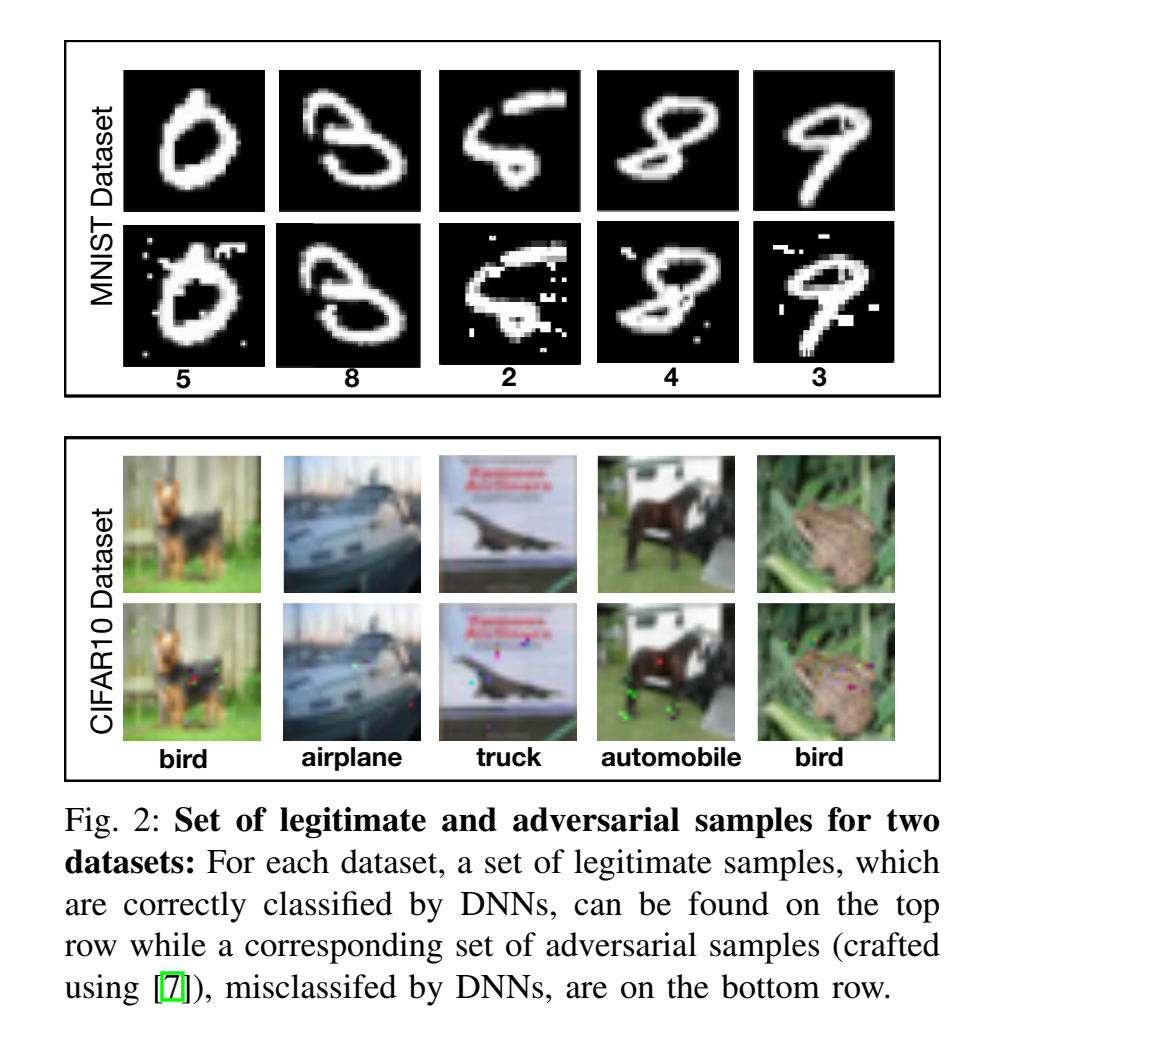
\includegraphics[scale=.42]{error}
\end{center}
\end{figure}
\noindent At presence of malicious data, the network can not only fail to generate proper outcome, they can also be manipulated to generate outcomes in accordance with the intent of the adversary. As the use of Deep Neural Network is widespread and many highly sensitive work is performed using Deep Neural Network, any adversarial attack can have devastating outcome. For example, Deep Learning algorithms are used in autonomous car driving algorithms. These industries require high precision for safety and functionality of cars on roads. Therefore, even a small number of malicious data sample, can cause the network to generate harmful outcome such as misidentifying a car or pedestrian for object or cat. Another example would be, bio-metric authentication systems. If the training is based on malicious data, they can be manipulated to allow improper access.
In this paper, they------------ have introduced a defensive mechanism called defensive distillation to reduce the effectiveness of adversarial samples on DNNs.\\\\
\noindent Distillation is a training procedure designed to train a DNN using knowledge transferred from a different DNN. Distillation reduces the complexity by transferring knowledge from big network to small network. This enables deployment of DL in smaller devices which are limited in computational resources. In this paper, authors formulated a variant of distillation to support defense training.  Instead of transferring knowledge between different architectures, they proposed to use the knowledge extracted from a DNN to improve its own resilience to adversarial samples[]. In this paper, they have tried to proof against the adversarial attack by avoiding high gradient amplitude in network for input samples by smoothing the gradient for all input and hence generalizing the network using knowledge gathered from distillation process. By reducing high gradient amplitude in input samples, they have reduced gradient amplitude in adversarial input sample data. This makes adversarial attack less effective as low gradient can not produce high variation in output and requires high number on malicious sample data to create harmful effect. This also generalizes the network and works well for new unknown data.\\\\
Distillation works as a security countermeasure against adversarial attack. This procedure generates smoother classifier models and reduces sensitivity
to input perturbations. The smother models are prone to be more resilient against adversarial samples. In this paper, they have shown empirically that defensive distillation reduces the success rate of adversarial sample crafting from 95:89\% to 0:45\% against a first DNN trained on the
MNIST dataset, and from 87:89\% to 5:11\% against a second DNN trained on the CIFAR10 dataset\cite{paper}.
\section*{Deep Neural Networks Architectures}
DNN network is composed of smaller units called neurons connected in hierarchical manner to produce a complex representations of a high dimensional input. In DNN there are input layer, two or more hidden layers and output layer. The input is is a vector representation of the input data which is fed into the input layer. Input layer may have some cell weights and biases applied on the input data, then the input from each neuron is transferred to following hidden layers. Each neuron in hidden layer has some weight, biases. After applying the weight and biases on the input from previous layer, the hidden layer apply activation function to produce output which is sent to the next hidden layer. All the successive hidden layer does the similar action to produce output for next layer. After output of the last hidden layer is passed to the output layer, the output layer may apply a function to produce output. Then the error is calculated and based on the calculation, the network weights are adjusted by back-propagating error. After intended number of repeating forward and backward propagation, the network is fully trained. This is a general architecture of DNN. There are couple of variation of DNN architecture. Depending on the activation function, learning rate and other hyper-parameter, network can behave differently.
\begin{figure}[H]
\begin{center}
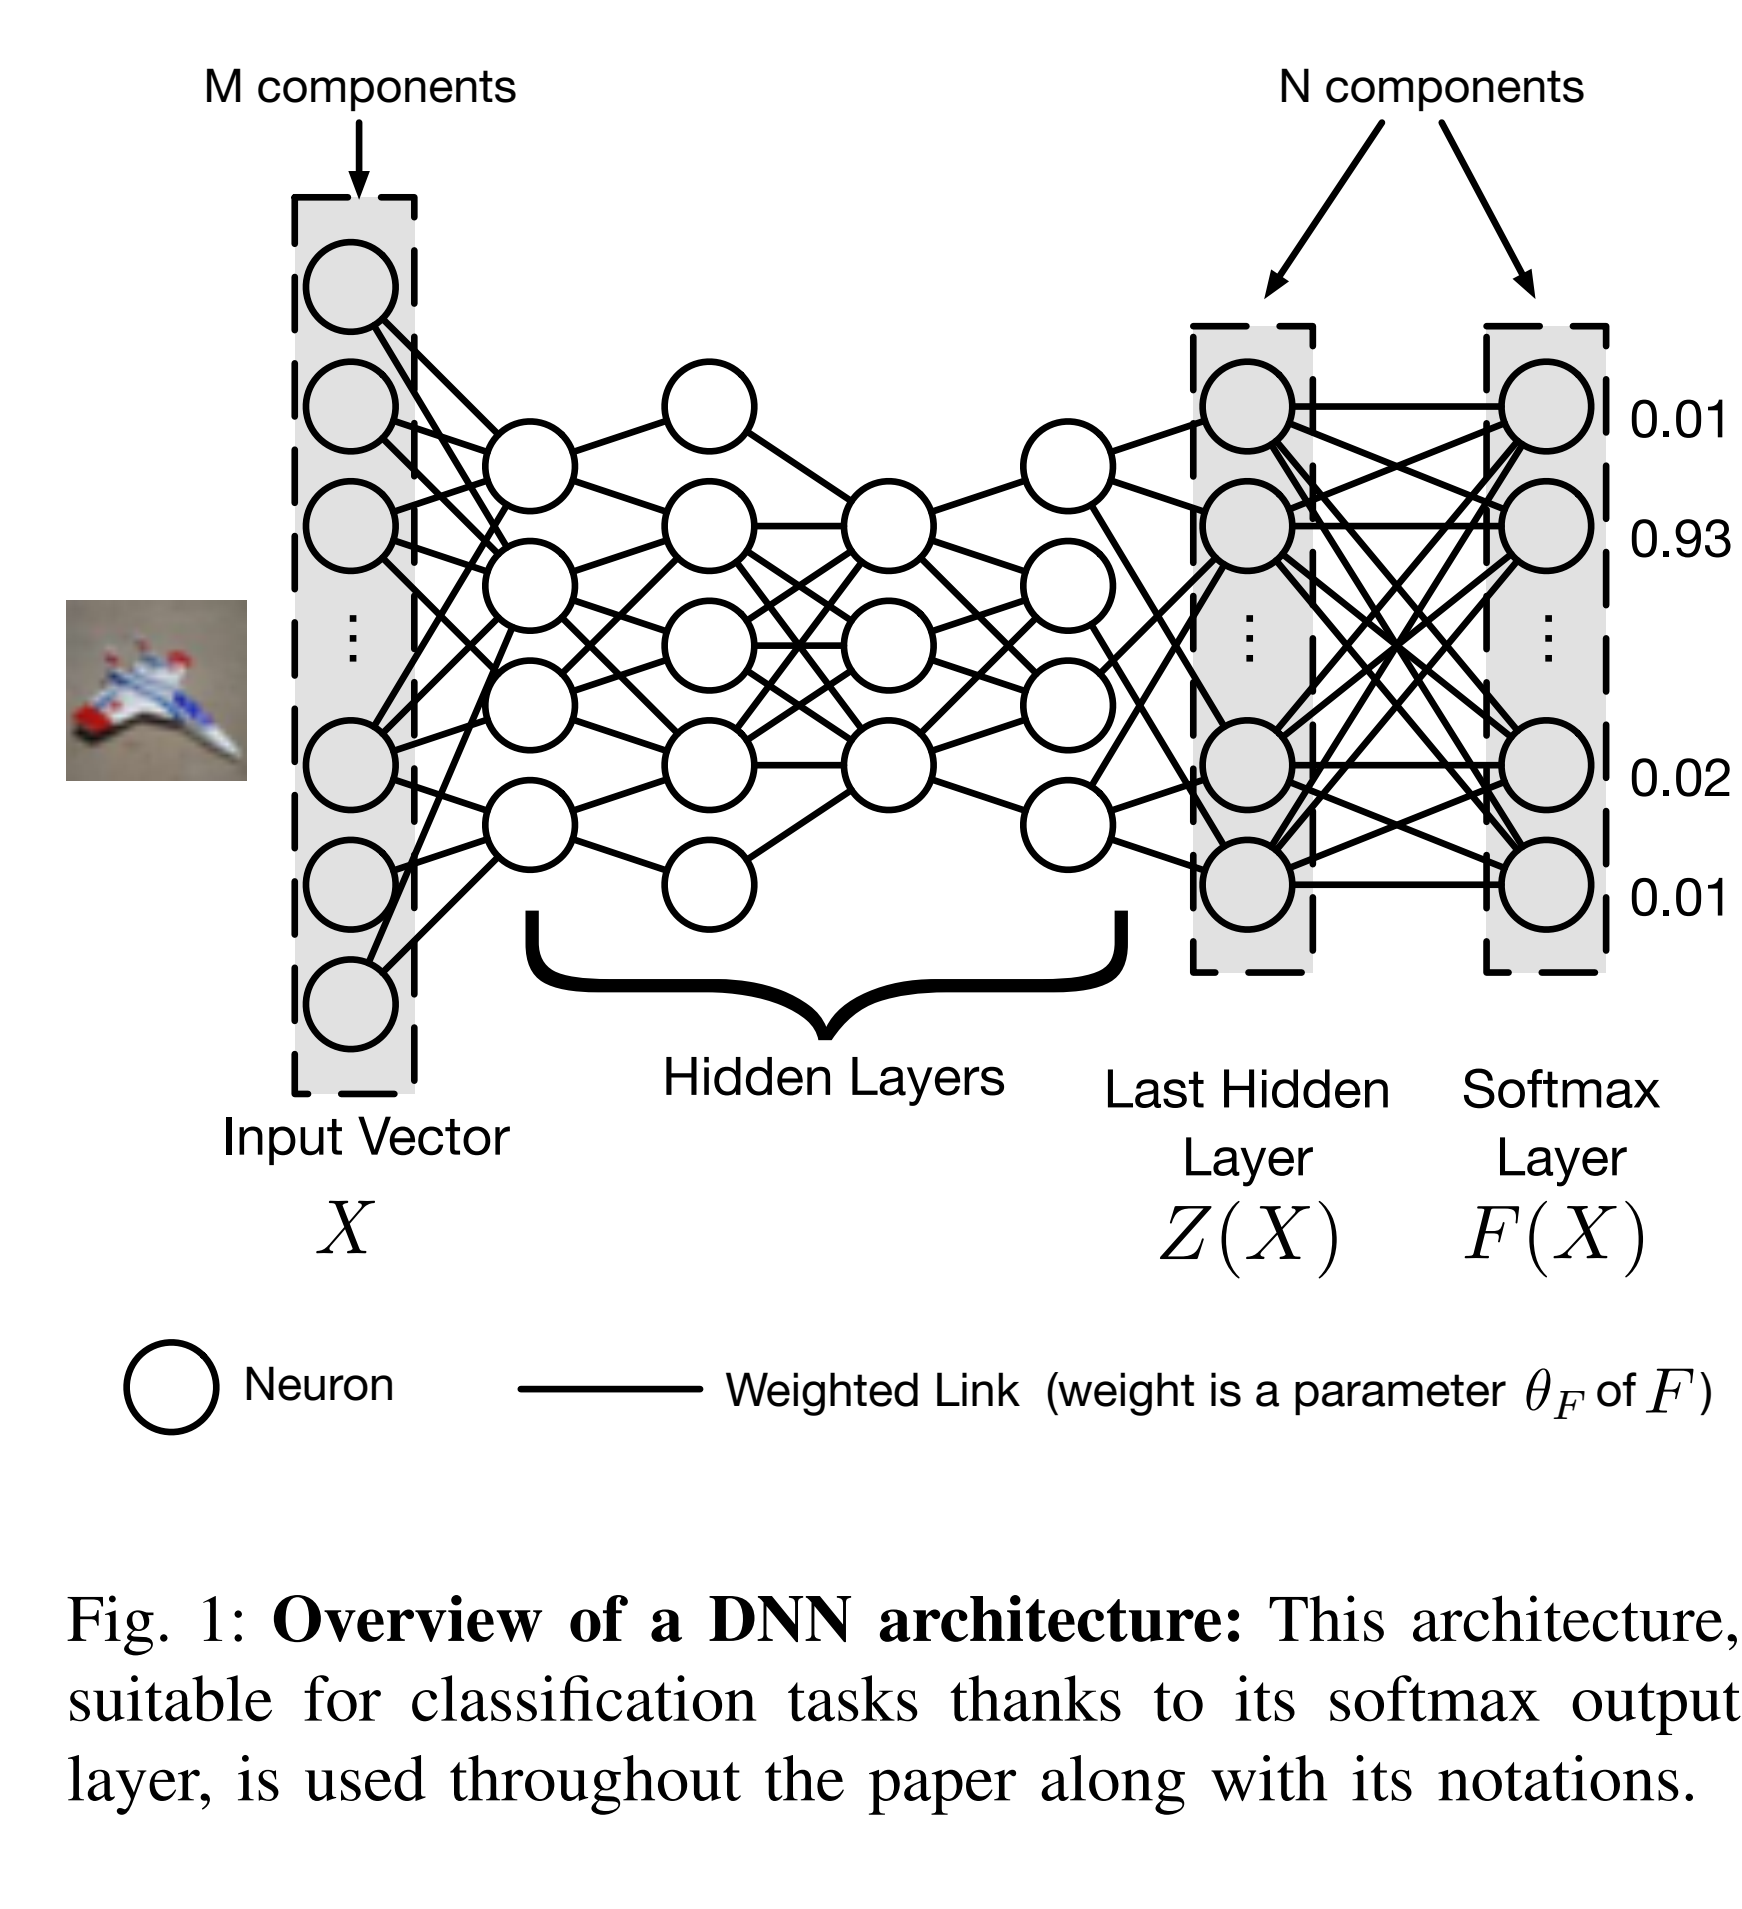
\includegraphics[scale=.2]{dnn}
\end{center}
\end{figure} 
\section*{Deep Adversarial Networks Architectures}
In deep Adversarial attack, the attacker may have capacity to induce ambuiguity. There is even more malicious from of DNN perturbation, in which advarsary will try to provoke network to output a target classification. This is specially hazarous. When system build on DNN, for example, digit recognition using Convolutional Neural Network (CNN), in presence of attack can misidentify digits and hence allow unintended access. Also, in financial system, even a fraudulent transaction may not raise alarm due to classyfying it as safe.  
\subsection*{Adversarial Input Crafting}
The adversarial sample crafting is then a two-step process:
\begin{enumerate}
\item Direction Sensitivity Estimation: evaluate the sensitivity
of class change to each input feature
\item Perturbation Selection: use the sensitivity information to
select a perturbation $\delta X$ among the input dimensions
\end{enumerate}
\begin{figure}[H]
\begin{center}
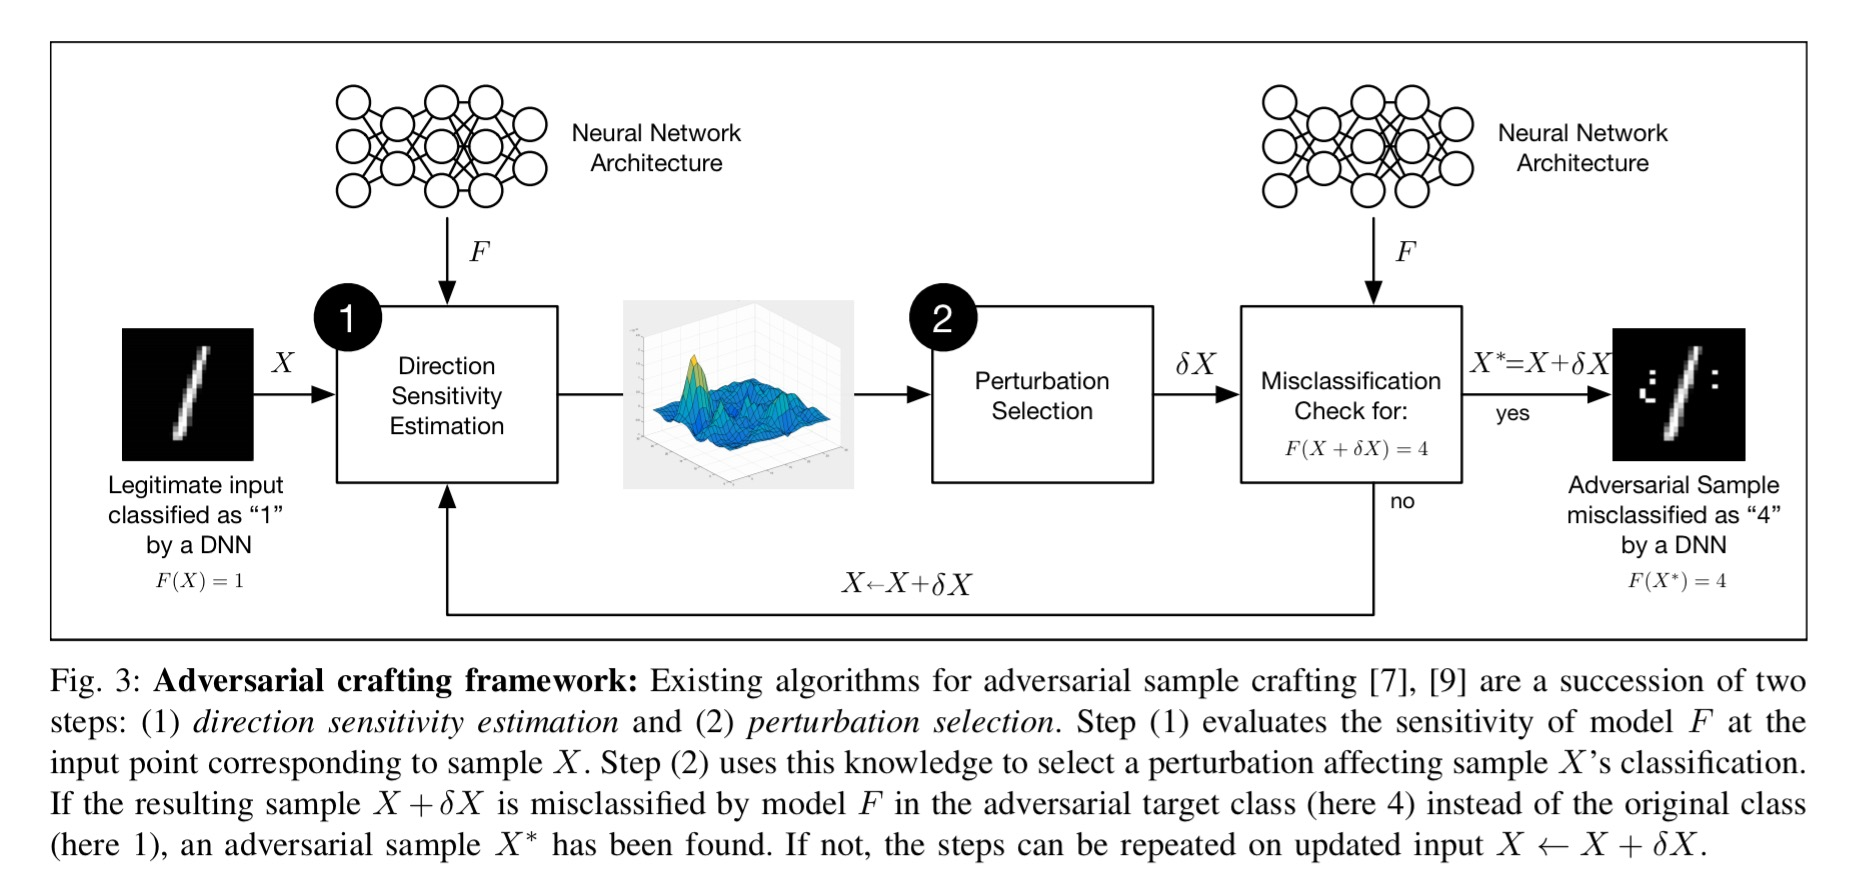
\includegraphics[scale=.25]{distillation-defense-fig-3}
\end{center}
\end{figure} 
The adversarial inputs are formulated using the original sample data. The sample input data samples perturbed such that it produces desired output with minimum change. Here the sensitivity off data is important which can give insight on how to change the input sample to produce maximum perturbation in network with least change of input data in right direction.
\subsubsection*{Direction Sensitivity Estimation}
The goal is finding the dimensions of inputs which will produce the expected adversarial output with the smallest perturbation\cite{paper}. For this the DNN model sensitivity to input has to be known. There are several ways model sensitivity to input can be leaned. On e process is, the fast sign
gradient method which calculates the gradient of the cost function
with respect to the input of the neural network. Finding
sensitivities is then achieved by applying the cost function
to inputs labeled using adversarial target labels\cite{paper}. Another method is forward derivative, which is the Jacobian of F, thus directly providing gradients of the output components with respect to each input
component\cite{paper}. There are many other sensitivity detection algorithms which can give direction sensitivity for model.
\subsubsection*{Perturbation Selection}
After gaining the knowledge of direction sensitivity of input for model, the adversary now can use this knowledge to perturb the DNN. This can be achieved by changing all the input dimension vectors in small scale and hence inducing shift to target outcome for the model. Another approach is to findi the minimal number of features to perturb in order to gain maximum shift to target outcome for the model. In both cases, efficiently of perturbation is calculated by the total change of the input vector.
\subsubsection*{About Neural Network Distillation}
For Neural Network Distillation process, authors have trained two DNN networks. First DNN network is trained using all the original input data smaples to produce probability class vector for each class. Then, the second DNN which is much smaller in size is trained using raw input data, class probability vector along with hard class labels. This generates more accurate DNN model, as the class probability is also taken into account. This works specially well when network is trained on devices with high resource constraint.\\\\
By making the model smoother and class space more smooth and wide, it can ensure that the network is more robust as input has natural distribution whereas adversarial input is crafted. For defense requirements low impact on the architecture, maintaining accuracy and speed of network is important. Also, defenses should work for adversarial samples relatively
close to points in the training dataset.
\begin{figure}[H]
\begin{center}
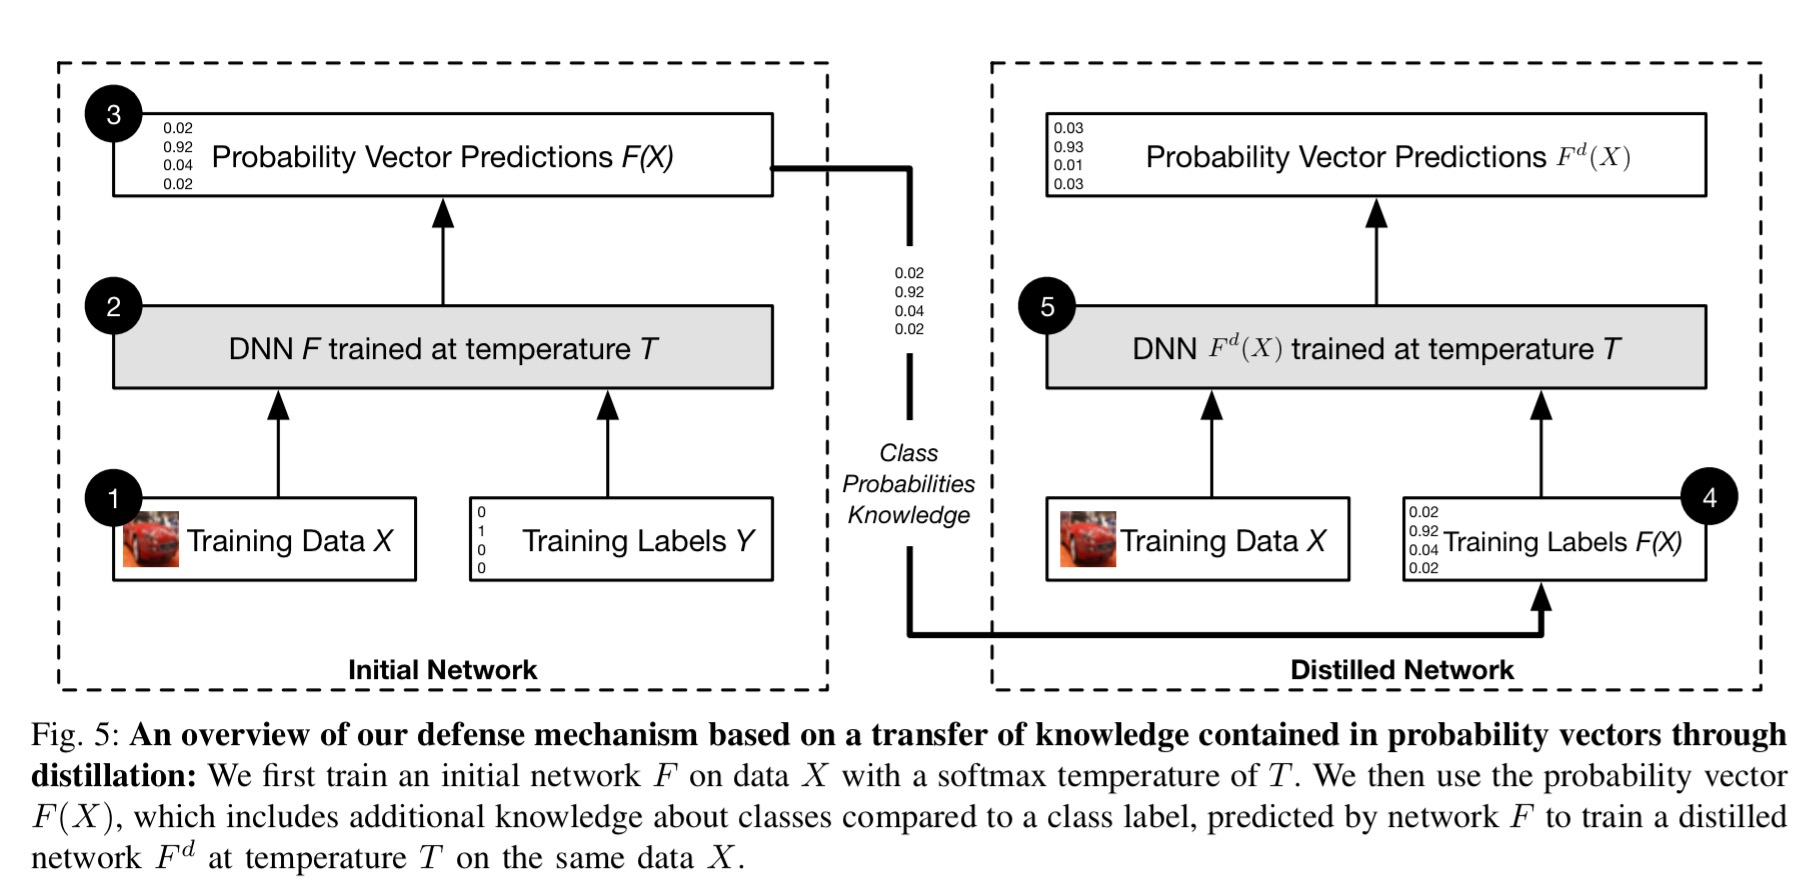
\includegraphics[scale=.22]{distillation-defense-fig-5}
\end{center}
\end{figure} 
\section*{Evaluation\cite{paper}}
Distillation reduces the success rate of adversarial crafting from 95:89\% to 0:45\% on our first DNN and dataset, and from 87:89\% to 5:11\% on a second DNN and dataset. Distillation has negligible or non existent degradation in model classification accuracy in these settings.Indeed the accuracy variability between models trained without distillation and with
distillation is smaller than 1:37\% for both DNNs.\\\\
Defensive distillation reduces DNN sensitivity to input perturbations, where
experiments show that performing distillation at high temperatures can lead to decreases in the amplitude of adversarial gradients by factors up to 1030.\\
Defensive distillation impacts the average minimum percentage of input features to be perturbed to achieve adversarial targets. In our DNNs, distillation increases robustness by 790\% for the first DNN and 556\% for the second DNN.
\section*{Overview of the Experimental Setup}
\subsection*{Dataset Description\cite{paper}}
two canonical machine learning datasets: the MNIST and CIFAR10 datasets.
The MNIST dataset is a collection of 70, 000 black and white images of handwritten digits, where each pixel is encoded as a real number between 0 and 1. The samples are split between a training set of 60, 000 samples and a test set of 10, 000. The classification goal is to determine the digit written. The classes therefore range from 0 to 9.\\\\
The CIFAR10 dataset is a collection of 60, 000 color images. Each pixel is encoded by 3 color components, which after preprocessing have values in
[-2.22, 2.62] for the test set. The samples are split between a training set of 50, 000 samples and a test set of 10, 000 samples. The images are to be classified in one of the 10 mutually exclusive classes: airplane, automobile, bird, cat, deer, dog, frog, horse, ship, and truck.\\
Some representative samples from each dataset are shown.
\begin{figure}[H]
\begin{center}
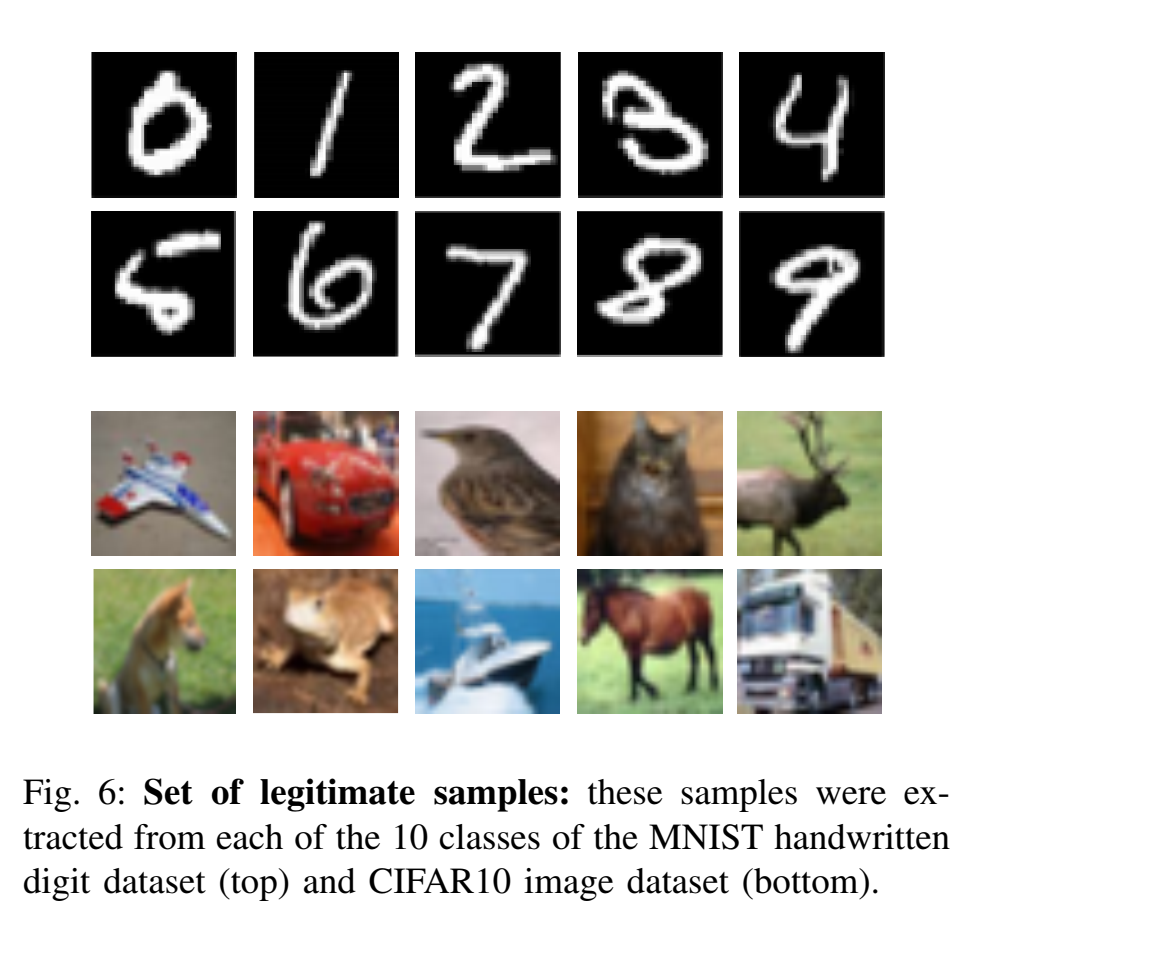
\includegraphics[scale=.5]{data}
\end{center}
\end{figure} 
\subsection*{Architecture Characteristics\cite{paper}}
The MNIST architecture is constructed using 2 convolutional
layers with 32 filters followed by a max pooling layer,
2 convolutional layers with 64 filters followed by a max
pooling layer, 2 fully connected layers with 200 rectified linear
units, and a softmax layer for classification in 10 classes. The
experimental DNN is trained on batches of 128 samples with
a learning rate of $\eta $ = 0.1 for 50 epochs. The resulting DNN
achieves a 99.51\% correct classification rate on the data set,
which is comparable to state-of-the-art DNN accuracy.
The CIFAR10 architecture is a succession of 2 convolutional
layers with 64 filters followed by a max pooling layer, 2 convolutional
layers with 128 filters followed by a max pooling
layer, 2 fully connected layers with 256 rectified linear units,
and a softmax layer for classification. When trained on batches
of 128 samples for the CIFAR10 dataset with a learning rate
of $\eta $= 0.01 (decay of 0.95 every 10 epochs), a momentum of
0.9 (decay of 0.5 every 10 epochs) for 50 epochs, a dropout
rate of 0.5, the architecture achieves a 80.95\% accuracy on
the CIFAR10 test set, which is comparable to state-of-the-art
performance for unaugmented datasets.
\begin{figure}[H]
\begin{center}
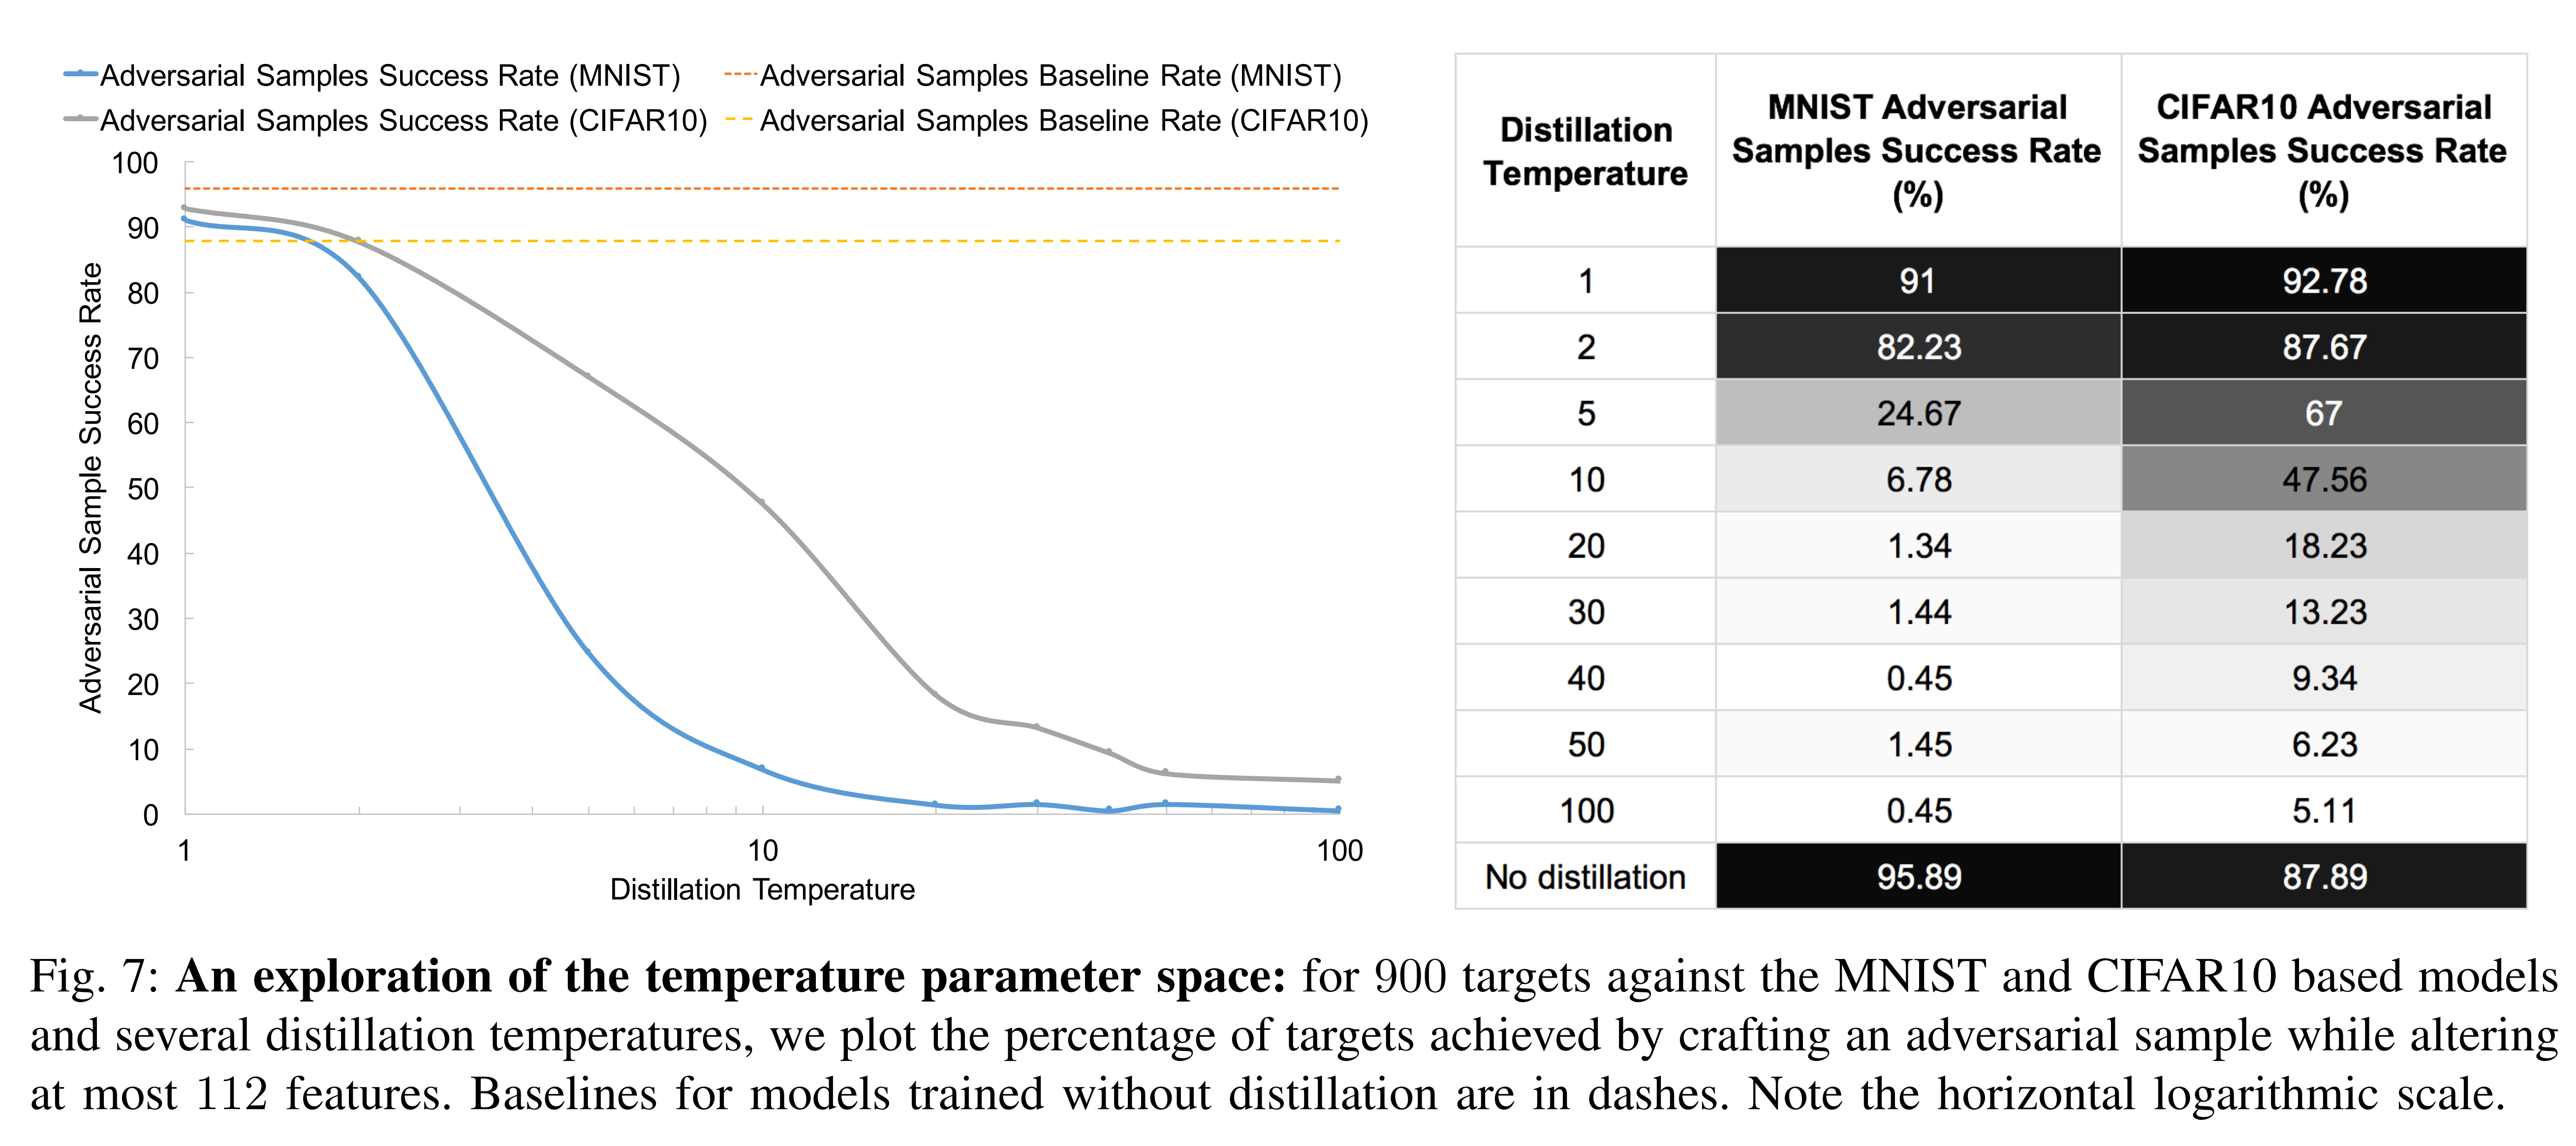
\includegraphics[scale=.15]{performance}
\end{center}
\end{figure}  
\begin{figure}[H]
\begin{center}
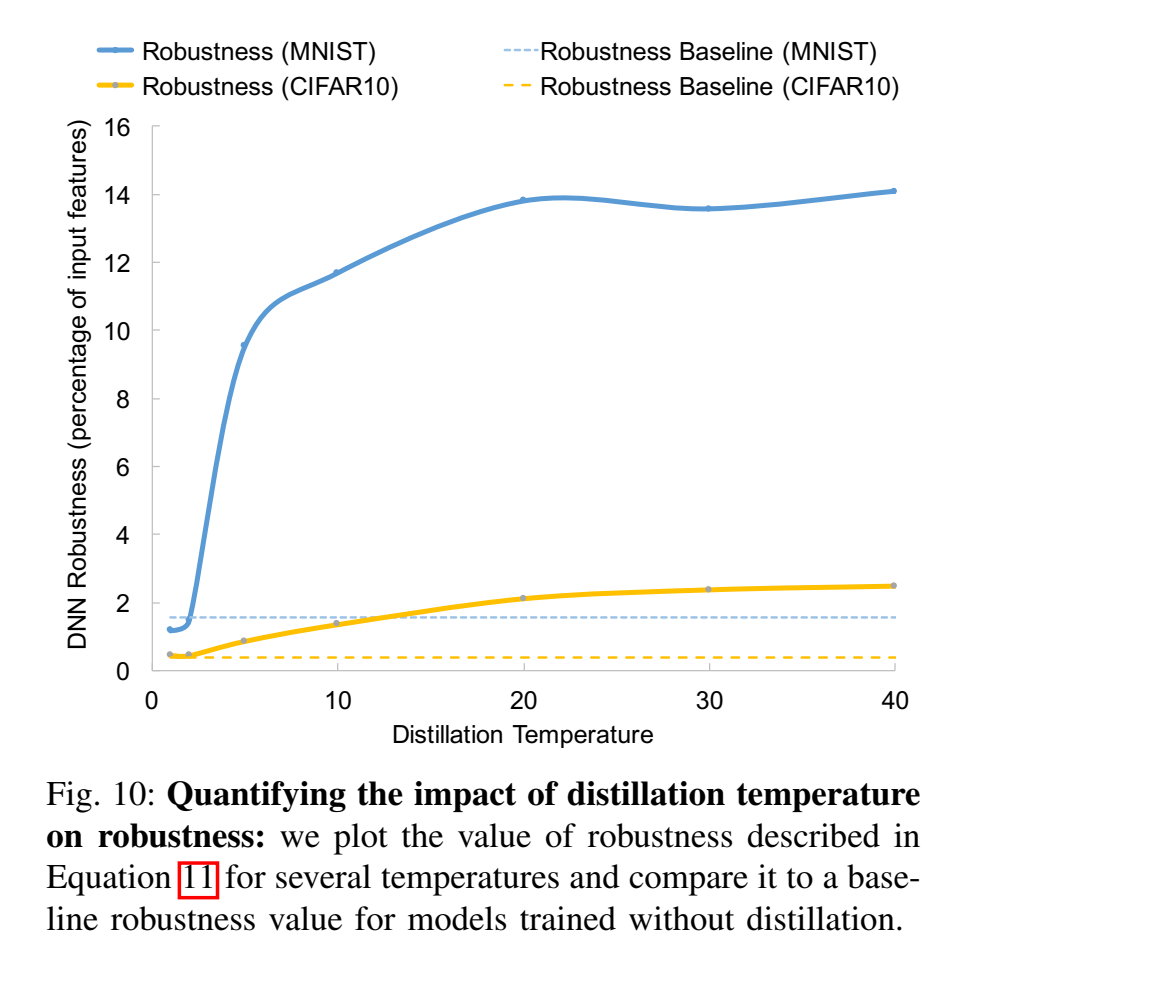
\includegraphics[scale=.4]{robust}
\end{center}
\end{figure} 
\section*{Conclusion}
Although the paper has empirically shown that using Neural Distillation for Deep Neural Network training can reduce target class adversarial attack, and better generalizes model by smoothing the gradient and reducing gradient amplitude variation for malicious input sample, hence reducing their impact to harm the DNN model, yet the authors are yet to conclude that the distillation process can be enough for defense against target class attack.
\begin{thebibliography}{}
\bibitem{paper} 
Papernot N, McDaniel P, Wu X, Jha S, Swami A. Distillation as a defense to adversarial perturbations against deep neural networks. InSecurity and Privacy (SP), 2016 IEEE Symposium on 2016 May 22 (pp. 582-597). IEEE.
\bibitem{mnist}
\textit{MNIST Database} 
\url{http://yann.lecun.com/exdb/mnist/}
\bibitem{cifar} 
\textit{CIFAR Dataset} 
\url{https://www.cs.toronto.edu/~kriz/cifar.html}
\end{thebibliography}
\end{document}

